

    \documentclass[table ]{article}

    \usepackage{graphicx}			% Use this package to include images
    \usepackage{amsmath}			% A library of many standard math expressions
    \usepackage[margin=0.75in, a4paper]{geometry}% Sets 1in margins. 
    \usepackage{fancyhdr}			% Creates headers and footers
    \usepackage{enumerate}          %These two package give custom labels to a list
    \usepackage[shortlabels]{enumitem}
    \usepackage{tikz}
    \usepackage{float} % Add this in your preamble for using [H]
    \usepackage{subcaption}
    \usepackage{booktabs}
    \usepackage{caption}
    \usepackage[normalem]{ulem}
    \useunder{\uline}{\ul}{}
    \usepackage{circuitikz}
    \usepackage{ragged2e} % Package for justification
    \justifying
    \usetikzlibrary{arrows}

    \graphicspath{{img/}}
    \usetikzlibrary{shapes.geometric, arrows, positioning}

    \def\mytitle{Homework 5}
    \def\righthead{EEF205E}


    \usepackage[T1]{fontenc}
    \usepackage{lmodern}

    \usepackage{listings}
    \usepackage{xcolor}
    \usepackage{colortbl}
    \usepackage{svg}
    \usepackage{ifthen}
    \usepackage{tikz}
    \usepackage{karnaugh-map}
    \usepackage{hyperref}

    \usetikzlibrary{calc}




    \pgfkeys{
    /sevenseg/.is family, /sevenseg,
    slant/.estore in      = \sevensegSlant,     % vertical slant in degrees
    size/.estore in       = \sevensegSize,      % length of a segment
    shrink/.estore in     = \sevensegShrink,    % avoids overlapping of segments
    line width/.estore in = \sevensegLinewidth, % thickness of the segments
    line cap/.estore in   = \sevensegLinecap,   % end cap style rect, round, butt
    oncolor/.estore in    = \sevensegOncolor,   % color of an ON segment
    offcolor/.estore in   = \sevensegOffcolor,  % color of an OFF segment
    }

    \pgfkeys{
    /sevenseg,
    default/.style = {slant = 0, size = 1em, shrink = 0.1, 
                        line width = 0.15em, line cap = round, 
                        oncolor = red, offcolor = lightgray}
    }




    %%%%%%%%%%%%%%%%%%%%%%%%%%%%%%%%%%%%%%%%%%%%%%%%%%%%%%%%
    \pagestyle{fancy}
    \fancyhead[l]{Rüzgar Erik}
    \fancyhead[c]{\mytitle}
    \fancyhead[r]{\righthead}
    \fancyfoot[c]{\thepage}
    \renewcommand{\headrulewidth}{0.2pt}
    \setlength{\headheight}{15pt}
    %%%%%%%%%%%%%%%%%%%%%%%%%%%%%%%%%%%%%%%%%%%%%%%%%%%%%%%%
    \usepackage{parskip}
    \setlength{\parindent}{0pt} % Disable paragraph indentation
    %%%%%%%%%%%%%%%%%%%%%%%%%%%%%%%%%%%%%%%%%%%%%%%%%%%%%%%%
    \usetikzlibrary{arrows,automata,positioning}




    \lstdefinestyle{vhdlstyle}{
        language=VHDL,
        backgroundcolor=\color{white},
        basicstyle=\ttfamily,
        keywordstyle=\color{blue},
        commentstyle=\color{green},
        stringstyle=\color{red},
        numbers=left,
        numberstyle=\tiny\color{gray},
        stepnumber=1,
        numbersep=5pt,
        tabsize=2,
        showspaces=false,
        showstringspaces=false,
    }



    \hypersetup{
    pdfauthor={Rüzgar Erik},
    pdftitle={\mytitle},
    pdfsubject={\righthead},
    pdfcreator={LaTeX},
    pdfproducer={Rüzgar Erik}
    }






    \begin{document}


    \begin{titlepage}
        \begin{figure}[h] % Places the figure at the right
            \begin{flushright}
            \includegraphics[width=0.3\textwidth]{logo_laci.png} % Change to your image name
                
            \end{flushright}
            \hfill
        \end{figure}

        \centering
        \vspace*{1in}
        
        \Huge
        \textbf{Introduction to Logic Design} \\
        \textbf{EEF205E} \\

        \vspace{0.5in}

        \Large
        \textbf{\mytitle} \\
        
        \vspace{0.5in}

        \large
        \textbf{Rüzgar Erik} \\
        \textbf{040240783} \\

        \vspace{0.5in}
        
        \Large
        Istanbul Technical University \\
        Faculty of Electrical and Electronics Engineering \\

        \vspace{0.25in}

        \today

        \vfill


    \end{titlepage}


    \section*{Question 1}

    Recalling the JK flip-flop equations we can derive  \(A(t+1)\) and \(B(t+1)\) as follows:

    \begin{equation}
        Q(t + 1) = J \cdot \overline{Q} + \overline{K} \cdot Q
    \end{equation}

    For the A flip-flop: \(J_A = x\) and \(K_A = b\)

    \begin{equation}
        A(t + 1) = x \cdot \overline{A} + \overline{b} \cdot A
    \end{equation}

    For the B flip-flop: \(J_B = x \) and \(K_B = \overline{a}\)

    \begin{equation}
        B(t + 1) = x \cdot \overline{B} + a \cdot B
    \end{equation}

    Given that there are 2 flip-flops there are \(2^2 = 4\) states and we can write the state transition table as follows:

    \begin{table}[H]
        \centering
        \caption{State Transition Table}
        \begin{tabular}{|c|c|c|c|c|c|c|}
            \hline
            \multicolumn{3}{|c|}{Present State} & \multicolumn{2}{c|}{Next State} \\
            \hline
            A & B &x& A(t+1) & B(t+1)  \\
            \hline
            0 & 0 & 0 & 0 & 0 \\
            0 & 0 & 1 & 1 & 1 \\
            \hline
            0 & 1 & 0 & 0 & 0 \\
            0 & 1 & 1 & 1 & 0 \\
            \hline
            1 & 0 & 0 & 1 & 0 \\
            1 & 0 & 1 & 1 & 1 \\
            \hline
            1 & 1 & 0 & 0 & 1 \\
            1 & 1 & 1 & 0 & 1 \\

            \hline

            \hline
        \end{tabular}
    \end{table}


    We can draw the state diagram as follows:

    \begin{figure}[H]
        \begin{center}
            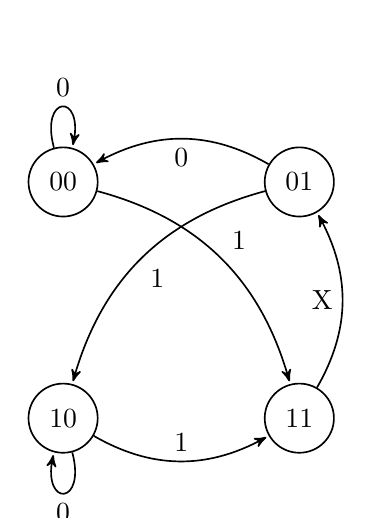
\begin{tikzpicture}[->,>=stealth',shorten >=1pt,auto,node distance=3cm,
                semithick]
                % Define the states as nodes
                \node[state] (A)                  {00};
                \node[state] (B) [right of=A]     {01};
                \node[state] (C) [below of=A]     {10};
                \node[state] (D) [below of=B]     {11};

                % Connect the states with arrows

                \path (A) edge [loop above] node {0} (A);
                \path (A) edge [bend left] node {1} (D);

                \path (B) edge [bend right] node {0} (A);
                \path (B) edge [bend right] node {1} (C);

                \path (C) edge [loop below] node {0} (C);
                \path (C) edge [bend right] node {1} (D);

                \path (D) edge [bend right] node {X} (B);

            \end{tikzpicture}
        \end{center}
        \caption{State Diagram}
    \end{figure}



    \newpage

    \section*{Question 2}

    The logic diagram for the state machine can be drawn as follows:



    \begin{figure}[H]
        \centering
        \includegraphics[width=\textwidth]{diagram1.png}     
        \caption{Logic Diagram for the State Machine}
    \end{figure}

    The state table can be written as follows:

    \begin{figure}[h]
        \centering
        \caption{State Table}
        \begin{tabular}{|c|c|c|c|c|c|c|}
            \hline
            \multicolumn{4}{|c|}{\textbf{Present State}} & \multicolumn{3}{c|}{\textbf{Next State}} \\
            \hline
            \textbf{A} & \textbf{B} & \textbf{x} & \textbf{y} & \textbf{A*} & \textbf{B*} & \textbf{z} \\ 
            \hline
            0 & 0 & 0 & 0 & 1 & 0 & 0 \\
            0 & 0 & 0 & 1 & 0 & 0 & 0 \\
            0 & 0 & 1 & 0 & 1 & 1 & 0 \\
            0 & 0 & 1 & 1 & 0 & 1 & 0 \\
            0 & 1 & 0 & 0 & 0 & 1 & 1 \\
            0 & 1 & 0 & 1 & 0 & 1 & 0 \\
            0 & 1 & 1 & 0 & 1 & 0 & 0 \\
            0 & 1 & 1 & 1 & 1 & 1 & 0 \\
            1 & 0 & 0 & 0 & 1 & 0 & 1 \\
            1 & 0 & 0 & 1 & 1 & 0 & 0 \\
            1 & 0 & 1 & 0 & 0 & 0 & 0 \\
            1 & 0 & 1 & 1 & 1 & 0 & 0 \\
            1 & 1 & 0 & 0 & 1 & 0 & 1 \\
            1 & 1 & 0 & 1 & 1 & 0 & 0 \\
            1 & 1 & 1 & 0 & 1 & 0 & 0 \\
            1 & 1 & 1 & 1 & 1 & 0 & 0 \\
        \hline
        \end{tabular}
    \end{figure}

    Recalling the JK flip-flop equations we can derive  \(A(t+1)\) and \(B(t+1)\) as follows:

    \begin{equation}
        Q(t + 1) = J \cdot \overline{Q} + \overline{K} \cdot Q
    \end{equation}


    For the A flip-flop: 

    \begin{equation}
        A^* = (b \cdot x + b' \cdot y') \cdot A' + (b + x' + y) \cdot A
    \end{equation}

    \begin{equation}
        B^* = (a' \cdot x) \cdot B' + [a' \cdot (x' + y)] \cdot B
    \end{equation}
    
    
\newpage



\section*{Question 3}

\textbf{Part A} \\


The state table for the requested circuit can be written as follows:

    
\begin{table}[H]
    \centering
    \caption{State Table}

    \begin{tabular}{|c|c|c|c|c|c|c|}
        \hline
        \multicolumn{3}{|c|}{Present State} & \multicolumn{2}{c|}{Next State} \\
        \hline
        A & B & x & A(t+1) & B(t+1)  \\
        \hline
        0 & 0 & 0 & 0 & 0 \\
        0 & 0 & 1 & 0 & 1 \\
        \hline
        0 & 1 & 0 & 0 & 1 \\
        0 & 1 & 1 & 1 & 1 \\
        \hline
        1 & 0 & 0 & 1 & 0 \\
        1 & 0 & 1 & 0 & 0 \\
        \hline
        1 & 1 & 0 & 1 & 1 \\
        1 & 1 & 1 & 1 & 0 \\
        \hline
\end{tabular}
\end{table}


To design the circuit with D Flip Flops We need its excitation table:

\begin{table}[H]
    \centering
    \caption{D Flip-Flop Excitation Table}
    \begin{tabular}{|c|c|c|c|}
        \hline
        Present State & Next State & D Input \\
        \hline
        0 & 0 & 0 \\
        0 & 1 & 1 \\
        1 & 0 & 0 \\
        1 & 1 & 1 \\
        \hline
    \end{tabular}
\end{table}


It can be seen that the equation for the D flip-flop is \(D = Q(t+1)\) so we can take the next state values from the state table and write the D values as follows:

\begin{table}[H]
    \centering
    \caption{State Table}

    \begin{tabular}{|c|c|c|c|c|c|c|c|c|}
        \hline
        \multicolumn{3}{|c|}{Present State} & \multicolumn{2}{c|}{Next State} & \multicolumn{2}{c|}{D Inputs}\\
        \hline
        A & B & x & A(t+1) & B(t+1) & D\_A & D\_B \\
        \hline
        0 & 0 & 0 & 0 & 0 & 0 & 0 \\
        0 & 0 & 1 & 0 & 1 & 0 & 1 \\
        \hline
        0 & 1 & 0 & 0 & 1 & 0 & 1 \\
        0 & 1 & 1 & 1 & 1 & 1 & 1 \\
        \hline
        1 & 0 & 0 & 1 & 0 & 1 & 0  \\
        1 & 0 & 1 & 0 & 0 & 0 & 0  \\
        \hline
        1 & 1 & 0 & 1 & 1 & 1 & 1 \\
        1 & 1 & 1 & 1 & 0 & 1 & 0 \\
        \hline
\end{tabular}
\end{table}


We can find equations for \(D_A\) and \(D_B\) with the help of kmaps:


\begin{figure}[H]
    \centering
    \begin{karnaugh-map}[2][4][1][$x$][$B$][$A$]
        \minterms{3,4,6,7}
        \maxterms{0,1,2,5}
        \implicant{3}{7}
        \implicant{6}{4}

    \end{karnaugh-map}
    \caption{K-Map for D\_A}
\end{figure}

The simplified equation for \(D_A\) is: 

\begin{equation}
D_A = (\overline{x_{in}} \cdot A) + (x_{in} \cdot B)
\end{equation}



We can draw the K-Map for \(D_B\) as follows:

\begin{figure}[H]
    \centering
    \begin{karnaugh-map}[2][4][1][$x$][$B$][$A$]
        \minterms{1,2,3,6}
        \maxterms{0,4,5,7}
        \implicant{2}{6}
        \implicant{1}{3}

    \end{karnaugh-map}
    \caption{K-Map for D\_B}
\end{figure}


The simplified equation for \(D_B\) is: 

\begin{equation}
    D_B = (\overline{x_{in}} \cdot B) + (x_{in} \cdot \overline{A})
\end{equation}


All of the equations can be implemented in a circuit as follows:

\begin{equation}
    D_A = (\overline{x_{in}} \cdot A) + (x_{in} \cdot B) 
\end{equation}

\begin{equation}
    D_B = (\overline{x_{in}} \cdot B) + (x_{in} \cdot \overline{A})
\end{equation}

\textbf{Part B} \\

The state table for the requested circuit can be written as follows:


\begin{table}[H]
    \centering
    \caption{State Table}

    \begin{tabular}{|c|c|c|c|c|c|c|}
        \hline
        \multicolumn{3}{|c|}{Present State} & \multicolumn{2}{c|}{Next State} \\
        \hline
        A & B & x & A(t+1) & B(t+1)  \\
        \hline
        0 & 0 & 0 & 0 & 0 \\
        0 & 0 & 1 & 1 & 1 \\
        \hline
        0 & 1 & 0 & 0 & 1 \\
        0 & 1 & 1 & 1 & 0 \\
        \hline
        1 & 0 & 0 & 1 & 0 \\
        1 & 0 & 1 & 0 & 0 \\
        \hline
        1 & 1 & 0 & 1 & 1 \\
        1 & 1 & 1 & 0 & 1 \\
        \hline
\end{tabular}
\end{table}

Again using the principle of D flip-flops we can add the D inputs to the state table as follows:





\begin{table}[H]
    \centering
    \caption{State Table}


    \begin{tabular}{|c|c|c|c|c|c|c|c|c|}
        \hline
        \multicolumn{3}{|c|}{Present State} & \multicolumn{2}{c|}{Next State} & \multicolumn{2}{c|}{D Inputs}\\
        \hline
        A & B & x & A(t+1) & B(t+1) & D\_A & D\_B \\
        \hline

        0 & 0 & 0 & 0 & 0 & 0 & 0 \\
        0 & 0 & 1 & 1 & 1 & 1 & 1 \\
        \hline
        0 & 1 & 0 & 0 & 1 & 0 & 1 \\
        0 & 1 & 1 & 1 & 0 & 1 & 0 \\
        \hline
        1 & 0 & 0 & 1 & 0 & 1 & 0 \\
        1 & 0 & 1 & 0 & 0 & 0 & 0 \\
        \hline
        1 & 1 & 0 & 1 & 1 & 1 & 1 \\
        1 & 1 & 1 & 0 & 1 & 0 & 1 \\
        \hline
\end{tabular}
\end{table}

We can find equations for \(D_A\) and \(D_B\) with the help of kmaps:


\begin{figure}[H]
    \centering
    \begin{karnaugh-map}[2][4][1][$x$][$B$][$A$]
        \minterms{1,3, 4, 6}
        \maxterms{0,2,5,7}
        \implicant{6}{4}
        \implicant{1}{3}

    \end{karnaugh-map}
    \caption{K-Map for D\_A}
\end{figure}

The simplified equation for \(D_A\) is:

\begin{equation}
    D_A = (\overline{x_{in}} \cdot A) + (x_{in} \cdot \overline{A})
\end{equation}

This shows an XOR gate is needed for the implementation of \(D_A\).

\begin{equation}
    D_A = x_{in} \oplus A
\end{equation}


We can draw the K-Map for \(D_B\) as follows:

\begin{figure}[H]
    \centering
    \begin{karnaugh-map}[2][4][1][$x$][$B$][$A$]
        \minterms{1,2,6,7}
        \maxterms{0,3,4,5}
        \implicant{2}{6}
        \implicant{1}{1}
        \implicant{7}{7}
    \end{karnaugh-map}
    \caption{K-Map for D\_B}
\end{figure}

The simplified equation for \(D_B\) is:

\begin{equation}
    D_B = (\overline{x_{in}} \cdot B) + (x_{in} \cdot \overline{B} \cdot \overline {A}) + (x_{in} \cdot A \cdot B)
\end{equation} 

Also it can be simplified with XNOR gates as follows:

\begin{equation}
    D_B = (\overline{x_{in}} \cdot B) + (x_{in} \cdot (A \odot B))
\end{equation}

So the circuit can be implemented as follows:

\begin{equation}
    D_A = x_{in} \oplus A
\end{equation}

\begin{equation}
    D_B = (\overline{x_{in}} \cdot B) + (x_{in} \cdot (A \odot B))
\end{equation}


\section*{Question 4}

For a serial 2s complementer, the circuit can be implemented as follows:\\
\(S_0 \) : We have not seen a 1 yet copy the input to the output 

\(S_1 \) : We have seen a 1, invert the output.

This is for LSB sent first approach.

The finite state machine can be implemented as follows:


\begin{figure}[H]
    \begin{center}
        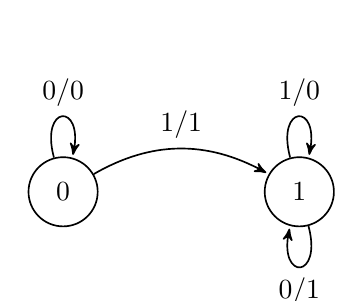
\begin{tikzpicture}[->,>=stealth',shorten >=1pt,auto,node distance=3cm,
            semithick]
            % Define the states as nodes
            \node[state] (A)                  {0};
            \node[state] (B) [right of=A]     {1};

            % Connect the states with arrows

            \path (A) edge [loop above] node {0/0} (A);
            \path (A) edge [bend left] node {1/1} (B);

            \path (B) edge [loop above] node {1/0} (B);
            \path (B) edge [loop below] node {0/1} (B);



        \end{tikzpicture}
    \end{center}
    \caption{State Diagram}
\end{figure}


The state table can be written as follows:

\begin{table}[H]
    \centering
    \caption{State Table}
    \begin{tabular}{|c|c|c|c|}
        \hline
        \multicolumn{2}{|c|}{Present State} & \multicolumn{2}{c|}{Next State} \\
        \hline
        Q & x & Q(t+1) & y  \\
        \hline
        0 & 0 & 0 & 0 \\
        0 & 1 & 1 & 1 \\
        1 & 0 & 1 & 1 \\
        1 & 1 & 1 & 0 \\
        \hline
    \end{tabular}
\end{table}

We are using D latch for this implementation. The D input can be written as follows:

It can be seen from the table that the D input it:

\begin{equation}
    D = Q + x
\end{equation}

And it can be seen that the y is the xor of the Q and x:

\begin{equation}
    y = Q \oplus x
\end{equation}

The circuit can be implemented as follows:

\begin{figure}[H]
    \centering
    \includegraphics[width=\textwidth]{diagram2.png}     
    \caption{Logic Diagram for the State Machine}
\end{figure}

\newpage

\section*{Question 5}

The requested state transition table is given in Table \ref{tab:state_transition}.

\begin{table}[H]
    \caption{State Transition Table for Sequential Circuit}
    \begin{center}
    \begin{tabular}{cccc|cc}
    \hline
    \multicolumn{2}{c}{Current State} & \multicolumn{2}{c|}{Inputs} & \multicolumn{2}{c}{Next State} \\
    A & B & E & F & A* & B* \\
    \hline
    0 & 0 & 0 & 0 & 0 & 0 \\
    0 & 0 & 0 & 1 & 0 & 0 \\
    0 & 0 & 1 & 0 & 1 & 1 \\
    0 & 0 & 1 & 1 & 0 & 1 \\
    \hline
    
    0 & 1 & 0 & 0 & 0 & 1 \\
    0 & 1 & 0 & 1 & 0 & 1 \\
    
    0 & 1 & 1 & 0 & 0 & 0 \\
    0 & 1 & 1 & 1 & 1 & 0 \\
    \hline
    
    1 & 0 & 0 & 0 & 1 & 0 \\
    1 & 0 & 0 & 1 & 1 & 0 \\
    
    1 & 0 & 1 & 0 & 0 & 1 \\
    1 & 0 & 1 & 1 & 1 & 1 \\
    \hline
    
    1 & 1 & 0 & 0 & 1 & 1 \\
    1 & 1 & 0 & 1 & 1 & 1 \\
    
    1 & 1 & 1 & 0 & 1 & 0 \\
    1 & 1 & 1 & 1 & 0 & 0 \\
    \hline
    \end{tabular}
    \end{center}
    \label{tab:state_transition}
    \end{table}


The state machine diagram can be drawn as follows:

\begin{figure}[H]
    \begin{center}
        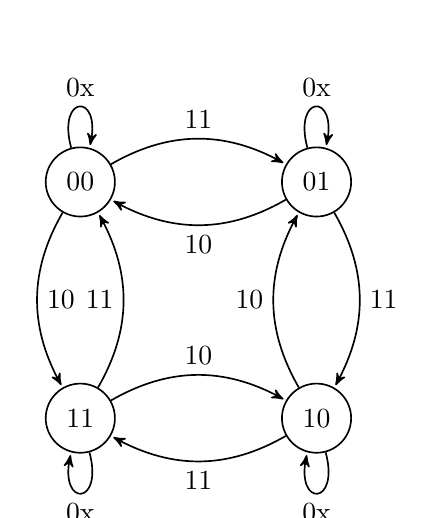
\begin{tikzpicture}[->,>=stealth',shorten >=1pt,auto,node distance=3cm,
            semithick]
            \node[state] (A)                  {00};
            \node[state] (B) [right of=A]     {01};
            \node[state] (D) [below of=A]     {11};
            \node[state] (C) [below of=B]     {10};

            % From A=00
            \path (A) edge[loop above] node {0x} (A);
            \path (A) edge[bend right]  node {10} (D);
            \path (A) edge[bend left]  node {11} (B);

            % From B=01

            \path (B) edge[loop above] node {0x} (B);
            \path (B) edge[bend left]  node {10} (A);
            \path (B) edge[bend left]  node {11} (C);

            % From C=10

            \path (C) edge[loop below] node {0x} (C);
            \path (C) edge[bend left]  node {10} (B);
            \path (C) edge[bend left]  node {11} (D);


            % From D=11

            \path (D) edge[loop below] node {0x} (D);
            \path (D) edge[bend left]  node {10} (C);
            \path (D) edge[bend right]  node {11} (A);


        \end{tikzpicture}
\end{center}
\caption{State Diagram}
\end{figure}


The E signal allows signal to change if its 0 F signal does not matter and the state does not change.

F = 1 counts up the state and F = 0 counts down the state.


The JK flip-flop equations can be written as follows:

\begin{equation}
    Q(t + 1) = J \cdot \overline{Q} + \overline{K} \cdot Q
\end{equation}

And the excitation table for the JK flip-flop can be written as follows:

\begin{table}[H]
    \centering
    \caption{JK Flip-Flop Excitation Table}
    \begin{tabular}{|c|c|c|c|}
        \hline
        Present State & Next State & J & K \\
        \hline
        0 & 0 & 0 & X \\
        0 & 1 & 1 & X \\
        1 & 0 & X & 1 \\
        1 & 1 & X & 0 \\
        \hline
    \end{tabular}
\end{table}


We can add 4 columns for \(J_A , J_B, K_A, K_B\)

\begin{table}[H]
    \caption{State Transition Table for Sequential Circuit}
    \begin{center}
    \begin{tabular}{cccc|cc|cc|cc}
    \hline
    \multicolumn{2}{c}{Current State} & \multicolumn{2}{c|}{Inputs} & \multicolumn{2}{c}{Next State} & \multicolumn{4}{c}{FF Inputs} \\
    A & B & E & F & A* & B* & J\_A & K\_A & J\_B & K\_B\\
    \hline
    0 & 0 & 0 & 0 & 0 & 0 & 0 & X & 0 & X \\
    0 & 0 & 0 & 1 & 0 & 0 & 0 & X & 0 & X \\
    0 & 0 & 1 & 0 & 1 & 1 & 1 & X & 1 & X \\
    0 & 0 & 1 & 1 & 0 & 1 & 0 & X & 1 & X \\
    \hline
    
    0 & 1 & 0 & 0 & 0 & 1 & 0 & X & X & 0 \\
    0 & 1 & 0 & 1 & 0 & 1 & 0 & X & X & 0 \\
    0 & 1 & 1 & 0 & 0 & 0 & 0 & X & X & 1 \\
    0 & 1 & 1 & 1 & 1 & 0 & 1 & X & X & 1 \\
    \hline
    
    1 & 0 & 0 & 0 & 1 & 0 & X & 0 & 0 & X \\
    1 & 0 & 0 & 1 & 1 & 0 & X & 0 & 0 & X \\
    1 & 0 & 1 & 0 & 0 & 1 & X & 1 & 1 & X \\
    1 & 0 & 1 & 1 & 1 & 1 & X & 0 & 1 & X \\
    \hline
    
    1 & 1 & 0 & 0 & 1 & 1 & X & 0 & X & 0 \\
    1 & 1 & 0 & 1 & 1 & 1 & X & 0 & X & 0 \\
    1 & 1 & 1 & 0 & 1 & 0 & X & 0 & X & 1 \\
    1 & 1 & 1 & 1 & 0 & 0 & X & 1 & X & 1 \\
    \hline
    \end{tabular}
    \end{center}
    \label{tab:state_transitio2}
    \end{table}

For finding the equations we can use kmaps:



\begin{figure}[H]
    \centering
    \begin{karnaugh-map}[4][4][1][$F$][$E$][$B$][$A$]
        % Indices 0..15 => 0,0,1,0, 0,0,0,1, X,X,X,X, X,X,X,X
        \manualterms{0,0,1,0, 0,0,0,1, X,X,X,X, X,X,X,X}
        % 1-cells at decimal 2 and 7
        \implicant{2}{2}
        \implicant{7}{7}
    \end{karnaugh-map}
    
    \caption{K-map for J\_A}
    \label{fig:kmap_ja}
\end{figure}


\begin{figure}[H]
    \centering
    \begin{karnaugh-map}[4][4][1][$F$][$E$][$B$][$A$]
        % Indices 0..15 => X,X,X,X, X,X,X,X, 0,0,1,0, 0,0,0,1
        \manualterms{X,X,X,X, X,X,X,X, 0,0,1,0, 0,0,0,1}
        % 1-cells at decimal 10 and 15
        \implicant{10}{10}
        \implicant{15}{15}
    \end{karnaugh-map}
    
    
    \caption{K-map for K\_A}
    \label{fig:kmap_ka}
    \end{figure}




% K-map for J_B
\begin{figure}[H]
    \centering
    \begin{karnaugh-map}[4][4][1][$F$][$E$][$B$][$A$]
        % Indices 0..15 => 0,0,1,1, X,X,X,X, 0,0,1,1, X,X,X,X
        \manualterms{0,0,1,1, X,X,X,X, 0,0,1,1, X,X,X,X}
        % 1-cells at decimal 2,3,10,11
        \implicant{3}{10}
    \end{karnaugh-map}
    
    
    \caption{K-map for J\_B}
    \label{fig:kmap_jb}
    \end{figure}


    % K-map for K_B
\begin{figure}[H]
    \centering
    \begin{karnaugh-map}[4][4][1][$F$][$E$][$B$][$A$]
        % Indices 0..15:
        %  0=X, 1=X, 2=X, 3=X,
        %  4=0, 5=0, 6=1, 7=1,
        %  8=X, 9=X, 10=X, 11=X,
        % 12=0, 13=0, 14=1, 15=1
        \manualterms{X,X,X,X, 0,0,1,1, X,X,X,X, 0,0,1,1}
        \implicant{3}{10}

        
        % Group (6,7) and (14,15).
    \end{karnaugh-map}
    
    \caption{K-map for K\_B}
    \label{fig:kmap_kb}
    \end{figure}


The final equations for the flip flops can be obtained from kmaps as follows:

\begin{equation}
    J_A = A'B \cdot (BF + B'F')
\end{equation}

\begin{equation}
    K_A = AE \cdot (BF + B'F')
\end{equation}

\begin{equation}
    J_B = E
\end{equation}

\begin{equation}
    K_B = E
\end{equation}


\section*{Part 2}

\subsection*{Question 1}
The Vhdl code for the requested circuit can be written as follows:

% import the code from code/1/JK_Latch.vhd

\begin{center} % Center the entire code block
    \lstset{
  caption= JK\_LATCH.vhd, 
  basicstyle=\footnotesize, frame=tb,
  xleftmargin=.2\textwidth, xrightmargin=.2\textwidth
}
    \lstinputlisting[style=vhdlstyle]{code/1/JK_Latch.vhd}
\end{center}

The testbench for the requested circuit can be written as follows:

% import the code from code/1/JK_Latch_tb.vhd

\begin{center} % Center the entire code block
    \lstset{
  caption= JK\_LATCH\_tb.vhd, 
  basicstyle=\footnotesize, frame=tb,
  xleftmargin=.2\textwidth, xrightmargin=.2\textwidth
}
    \lstinputlisting[style=vhdlstyle]{code/1/JK_Latch_tb.vhd}
\end{center}



The RTL schematic for the requested circuit can be seen in Figure \ref{fig:jk_latch_rtl}.

\begin{figure}[H]
    \centering
    \includegraphics[width=\textwidth]{img/1/rtl.png}
    \caption{RTL Schematic for JK Latch}
    \label{fig:jk_latch_rtl}
\end{figure}



The simulation results can be seen in Figure \ref{fig:jk_latch_sim}.

\begin{figure}[H]
    \centering
    \includegraphics[width=\textwidth]{img/1/sim.png}
    \caption{Simulation Results for JK Latch}
    \label{fig:jk_latch_sim}
\end{figure}


\section*{Question 2}

The Vhdl code for the requested circuit can be written as follows:

% import the code from code/2/JK_FF.vhd

\begin{center} % Center the entire code block
    \lstset{
  caption= JK\_FF.vhd, 
  basicstyle=\footnotesize, frame=tb,
  xleftmargin=.2\textwidth, xrightmargin=.2\textwidth
}
    \lstinputlisting[style=vhdlstyle]{code/2/JK_FF.vhd}
\end{center}

The testbench for the requested circuit can be written as follows:

% import the code from code/2/JK_FF_tb.vhd

\begin{center} % Center the entire code block
    \lstset{
  caption= JK\_FF\_tb.vhd, 
  basicstyle=\footnotesize, frame=tb,
  xleftmargin=.2\textwidth, xrightmargin=.2\textwidth
}
    \lstinputlisting[style=vhdlstyle]{code/2/JK_FF_tb.vhd}

\end{center}

The RTL schematic for the requested circuit can be seen in Figure \ref{fig:jk_ff_rtl}.

\begin{figure}[H]
    \centering
    \includegraphics[width=\textwidth]{img/2/rtl.png}
    \caption{RTL Schematic for JK Flip Flop}
    \label{fig:jk_ff_rtl}

\end{figure}

The simulation results can be seen in Figure \ref{fig:jk_ff_sim}.

\begin{figure}[H]
    \centering
    \includegraphics[width=\textwidth]{img/2/sim.png}
    \caption{Simulation Results for JK Flip Flop}
    \label{fig:jk_ff_sim}

\end{figure}


\section*{Question 3}

\begin{figure}[H]
    \begin{center}
        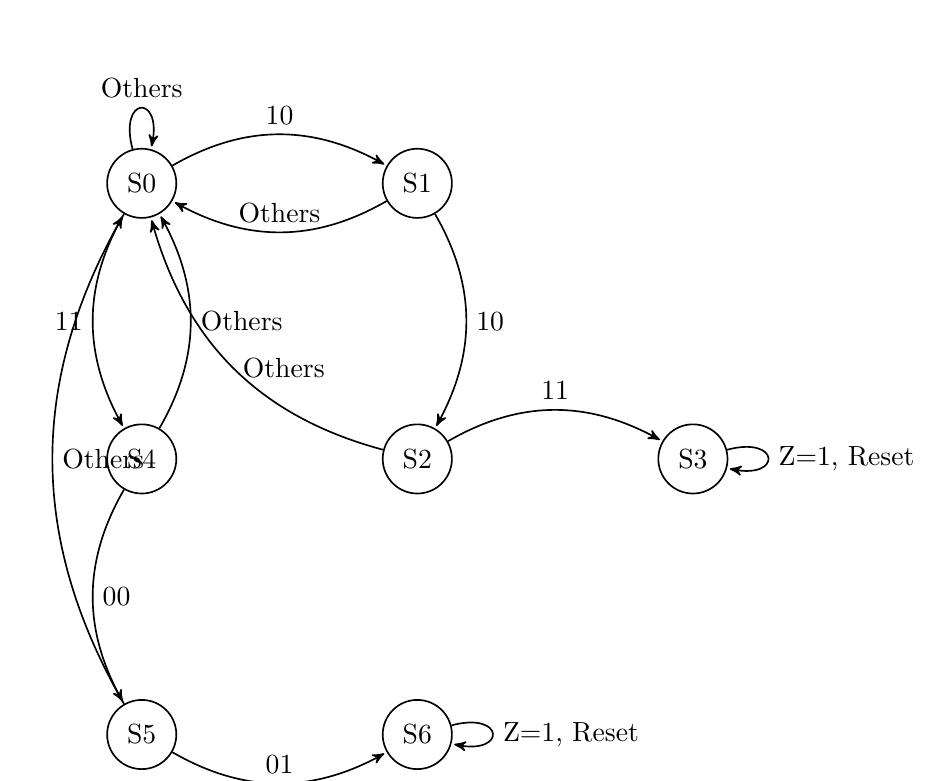
\begin{tikzpicture}[->,>=stealth',shorten >=1pt,auto,node distance=3.5cm,
            semithick]
            % Define the states as nodes
            \node[state] (S0)                  {S0};
            \node[state] (S1) [right of=S0]    {S1};
            \node[state] (S2) [below of=S1]    {S2};
            \node[state] (S3) [right of=S2]    {S3};
            \node[state] (S4) [below of=S0]    {S4};
            \node[state] (S5) [below of=S4]    {S5};
            \node[state] (S6) [right of=S5]    {S6};

            % Connect the states with arrows
            \path (S0) edge [bend left] node {10} (S1)
                        edge [bend right] node [left] {11} (S4)
                        edge [loop above] node {Others} (S0);

            \path (S1) edge [bend left] node {10} (S2)
                        edge [bend left] node [above] {Others} (S0);

            \path (S2) edge [bend left] node {11} (S3)
                        edge [bend left] node [right] {Others} (S0);

            \path (S3) edge [loop right] node {Z=1, Reset} (S0);

            \path (S4) edge [bend right] node {00} (S5)
                        edge [bend right] node [right] {Others} (S0);

            \path (S5) edge [bend right] node {01} (S6)
                        edge [bend left] node [right] {Others} (S0);

            \path (S6) edge [loop right] node {Z=1, Reset} (S0);
            

        \end{tikzpicture}
    \end{center}
    \caption{State Diagram for Pattern Detector}
\end{figure}


\begin{enumerate}
    \item \textbf{S0}: Initial state (waiting for a valid start of a pattern).
    \item \textbf{S1}: `10` detected (beginning of Pattern 1).
    \item \textbf{S2}: `10-10` detected (middle of Pattern 1).
    \item \textbf{S3}: `10-10-11` detected (Pattern 1 complete, \(Z = 1\)).
    \item \textbf{S4}: `11` detected (beginning of Pattern 2).
    \item \textbf{S5}: `11-00` detected (middle of Pattern 2).
    \item \textbf{S6}: `11-00-01` detected (Pattern 2 complete, \(Z = 1\)).
\end{enumerate}


The VHDL code for the requested circuit can be written as follows:

% import the code from code/3/Pattern_Detector.vhd

\begin{center} % Center the entire code block
    \lstset{
  caption= Pattern\_Detector.vhd, 
  basicstyle=\footnotesize, frame=tb,
  xleftmargin=.2\textwidth, xrightmargin=.2\textwidth
}
    \lstinputlisting[style=vhdlstyle]{code/3/Pattern_Detector.vhd}

\end{center}

The testbench for the requested circuit can be written as follows:


% import the code from code/3/Pattern_Detector_tb.vhd

\begin{center} % Center the entire code block
    \lstset{
  caption= Pattern\_Detector\_tb.vhd, 
  basicstyle=\footnotesize, frame=tb,
  xleftmargin=.2\textwidth, xrightmargin=.2\textwidth
}
    \lstinputlisting[style=vhdlstyle]{code/3/Pattern_Detector_tb.vhd}

\end{center}


The RTL schematic for the requested circuit can be seen in Figure \ref{fig:pattern_detector_rtl}.

\begin{figure}[H]
    \centering
    \includegraphics[width=\textwidth]{img/3/rtl.png}
    \caption{RTL Schematic for Pattern Detector}
    \label{fig:pattern_detector_rtl}

\end{figure}

The simulation results can be seen in Figure \ref{fig:pattern_detector_sim}.

\begin{figure}[H]
    \centering
    \includegraphics[width=\textwidth]{img/3/sim.png}
    \caption{Simulation Results for Pattern Detector}
    \label{fig:pattern_detector_sim}
\end{figure}



\section*{Question 4}

Assigning the states as follows:


\begin{table}[H]
    \centering
    \caption{State and Assignment Table}
    \begin{tabular}{|c|c|}
        \hline
        \textbf{State} & \textbf{$Q_2 Q_1 Q_0$} \\
        \hline
        $S_0$ & 000 \\
        \hline
        $S_1$ & 001 \\
        \hline
        $S_2$ & 010 \\
        \hline
        $S_3$ & 011 \\
        \hline
        $S_4$ & 100 \\
        \hline
        $S_5$ & 101 \\
        \hline
        $S_6$ & 110 \\
        \hline
    \end{tabular}
\end{table}

Using the excitation table of JK flip-flops, we can find the JK inputs for each state transition as follows:

\begin{table}[H]
    \centering
    \caption{JK Flip-Flop Excitation Table}
    \begin{tabular}{|c|c|c|c|}
        \hline
        Present State & Next State & J & K \\
        \hline
        0 & 0 & 0 & X \\
        0 & 1 & 1 & X \\
        1 & 0 & X & 1 \\
        1 & 1 & X & 0 \\
        \hline
    \end{tabular}
\end{table}



\begin{table}[H]
    \centering
    \renewcommand{\arraystretch}{1.5}
    \begin{tabular}{|c|c|c|c|c|c|c|}
    \hline
    \textbf{Current} $(Q_2 Q_1 Q_0)$ & \textbf{Input} $(A_1 A_0)$ & \textbf{Next} $(Q_2^+ Q_1^+ Q_0^+)$ & \textbf{Z} & $(J_2, K_2)$ & $(J_1, K_1)$ & $(J_0, K_0)$ \\ \hline
    $000~(S0)$ & $10$ & $001~(S1)$ & $0$ & $(0, X)$ & $(0, X)$ & $(1, X)$ \\ \hline
    $000~(S0)$ & $11$ & $100~(S4)$ & $0$ & $(1, X)$ & $(0, X)$ & $(0, X)$ \\ \hline
    $000~(S0)$ & Others & $000~(S0)$ & $0$ & $(0, X)$ & $(0, X)$ & $(0, X)$ \\ \hline
    $001~(S1)$ & $10$ & $010~(S2)$ & $0$ & $(0, X)$ & $(1, X)$ & $(X, 1)$ \\ \hline
    $001~(S1)$ & Others & $000~(S0)$ & $0$ & $(0, X)$ & $(0, X)$ & $(X, 1)$ \\ \hline
    $010~(S2)$ & $11$ & $011~(S3)$ & $1$ & $(0, X)$ & $(X, 0)$ & $(1, X)$ \\ \hline
    $010~(S2)$ & Others & $000~(S0)$ & $0$ & $(0, X)$ & $(X, 1)$ & $(0, X)$ \\ \hline
    $011~(S3)$ & Any & $000~(S0)$ & $0$ & $(0, X)$ & $(X, 1)$ & $(X, 1)$ \\ \hline
    $100~(S4)$ & $00$ & $101~(S5)$ & $0$ & $(X, 0)$ & $(0, X)$ & $(1, X)$ \\ \hline
    $100~(S4)$ & Others & $000~(S0)$ & $0$ & $(X, 1)$ & $(0, X)$ & $(0, X)$ \\ \hline
    $101~(S5)$ & $01$ & $110~(S6)$ & $1$ & $(X, 0)$ & $(1, X)$ & $(X, 1)$ \\ \hline
    $101~(S5)$ & Others & $000~(S0)$ & $0$ & $(X, 1)$ & $(0, X)$ & $(X, 1)$ \\ \hline
    $110~(S6)$ & Any & $000~(S0)$ & $0$ & $(X, 1)$ & $(X, 1)$ & $(0, X)$ \\ \hline
    \end{tabular}
    \caption{State Transition Table with JK Inputs}
    \label{tab:state-transition}
    \end{table}
    
    
The expressions were simplified and the results are
\[
\begin{aligned}
J_{2} &= \overline{Q_{2}}\,\overline{Q_{1}}\,\overline{Q_{0}}\,A_{1}\,A_{0},\\
K_{2} &= (Q_{2}Q_{1}) + (Q_{2}\,\overline{Q_{1}}\,\overline{Q_{0}}\,(A_{1}+A_{0})) + (Q_{2}\,\overline{Q_{1}}\,Q_{0}\,(A_{1}+\overline{A_{0}})),\\
J_{1} &= \overline{Q_{1}}\,Q_{0}\,\bigl(\overline{Q_{2}}\,A_{1}\,\overline{A_{0}} + Q_{2}\,\overline{A_{1}}\,A_{0}\bigr),\\
K_{1} &= \overline{Q_{2}}\,Q_{1}\,\overline{Q_{0}}\,(\overline{A_{1}}+\overline{A_{0}}) + \overline{Q_{2}}\,Q_{1}\,Q_{0} + Q_{2}\,Q_{1}\,\overline{Q_{0}},\\
J_{0} &= \overline{Q_{2}}\,\overline{Q_{1}}\,\overline{Q_{0}}\,A_{1}\,\overline{A_{0}} + \overline{Q_{2}}\,Q_{1}\,\overline{Q_{0}}\,A_{1}\,A_{0} + Q_{2}\,\overline{Q_{1}}\,\overline{Q_{0}}\,\overline{A_{1}}\,\overline{A_{0}},\\
K_{0} &= \overline{Q_{2}}\,\overline{Q_{1}}\,Q_{0}\,(\overline{A_{1}}+A_{0}) + \overline{Q_{2}}\,Q_{1}\,Q_{0} + Q_{2}\,\overline{Q_{1}}\,Q_{0},\\
Z &= \overline{Q_{2}}\,Q_{1}\,\overline{Q_{0}}\,A_{1}\,A_{0} + Q_{2}\,\overline{Q_{1}}\,Q_{0}\,\overline{A_{1}}\,A_{0}.
\end{aligned}
\]

The vhdl code for the requested circuit can be written as follows:

% import the code from code/4/Pattern_Detector_JK_FF.vhd

\begin{center} % Center the entire code block
    \lstset{
  caption= Pattern\_Detector\_JK\_FF.vhd, 
  basicstyle=\footnotesize, frame=tb,
  xleftmargin=.2\textwidth, xrightmargin=.2\textwidth
}
    \lstinputlisting[style=vhdlstyle]{code/4/Pattern_Detector_JK_FF.vhd}

\end{center}

The testbench for the requested circuit can be written as follows:

% import the code from code/4/Pattern_Detector_JK_FF_tb.vhd

\begin{center} % Center the entire code block
    \lstset{
  caption= Pattern\_Detector\_JK\_FF\_tb.vhd, 
  basicstyle=\footnotesize, frame=tb,
  xleftmargin=.2\textwidth, xrightmargin=.2\textwidth
}
    \lstinputlisting[style=vhdlstyle]{code/4/Pattern_Detector_JK_FF_tb.vhd}

\end{center}


The RTL schematic for the requested circuit can be seen in Figure \ref{fig:pattern_detector_jk_ff_rtl}.


\begin{figure}[H]
    \centering
    \includegraphics[width=\textwidth]{img/4/rtl.png}
    \caption{RTL Schematic for Pattern Detector with JK Flip-Flops}
    \label{fig:pattern_detector_jk_ff_rtl}
\end{figure}

The simulation results can be seen in Figure \ref{fig:pattern_detector_jk_ff_sim}.

\begin{figure}[H]
    \centering
    \includegraphics[width=\textwidth]{img/4/sim.png}
    \caption{Simulation Results for Pattern Detector with JK Flip-Flops}
    \label{fig:pattern_detector_jk_ff_sim}
\end{figure}




\end{document}


